\documentclass{beamer}
\usepackage{graphicx,color,amsmath,amssymb,amsfonts,amsbsy,amsthm}
% Node the following tag will orient things right using dvi2pdf.
% Process with LaTeX first, then dvi2pdf.
\special{landscape}
% Fuzz -----------------------------------------------------------
\hfuzz5pt % Don't bother to report overfull boxes < 5pt
% MATH -----------------------------------------------------------
\input{kalman_cmdmaster.tex}
% THEOREM ENV. ---------------------------------------------------
\newtheorem{thm}{Theorem.}
\newtheorem{cor}[thm]{Corollary.}
\newtheorem{con}[thm]{Conjecture.}
\newtheorem{lem}[thm]{Lemma.}
\newtheorem{prop}[thm]{Proposition.}
\newtheorem{defn}[thm]{Def inition.}
\renewcommand{\thethm}{}  % unnumbered
\pagestyle{plain}
%%% --------------------------------------------------------------
\begin{document}
\title{
\vfill \hrulefill \vfill
\begin{center}
Overview of Kalman Filter Theory and Navigation Applications\\
Day 4
\end{center}
}
\author{Michael L. Carroll}
\date{Feb 25, 2003\\
\vfill \hrulefill \vspace*{.25in} \vfill
\begin{tiny}
\copyright 2003 by Michael L. Carroll
\end{tiny}
} \maketitle
% ----------------------------------------------------------------
% day4_seg1_sim/sim_main.tex
\begin{frame}
\textbf{Day 4: General Code Implementation Issues\\
Topics}
 \begin{itemize}
 \item Simulation vs. Real-Time Implementation
 \item Survey of Navaids
 \item Filter Maintenance
 \item Filter Redundancy and Fault Tolerance
\end{itemize}
\end{frame}
\begin{frame}
\textbf{Day 4, Segment 1\\
Simulation vs. Real-Time Implementation\\
Topics }
\begin{itemize}
 \item Simulation
 \item Real-Time Implementation
\end{itemize}
\end{frame}
% day4_seg1_sim/simulation.tex
\begin{frame}
Simulation
 \begin{itemize}
 \item Introduction to Matlab / Simulink
 \item Covariance Analysis
 \item Trajectory Simulation
\end{itemize}
\end{frame}
\begin{frame}
Introduction to Simulink
\begin{itemize}
  \item Matlab
  \item Simulink
\end{itemize} 
\end{frame}

\begin{frame}
Matlab
\begin{itemize}
  \item Matrix-oriented scientfic computing tool from Mathworks
	\begin{itemize}
	  \item Everything is a matrix: scalars are 1-by-1 matrices
	\end{itemize}
  \item Lots of built-in numerical tools for matrix manipulation
  \item Industry standard
\end{itemize} 
\end{frame}

\begin{frame}[fragile]
Matlab
\begin{verbatim}
%   Row vector:
v = [1 2 3]; % Or separate columns with comma: v = [1, 2, 3];
%   Column vector:
u = [1;2;3]; % Note: Rows separated with semicolon
% Natural multiplication:
x=v*u;
\end{verbatim}

\end{frame}

\begin{frame}[fragile]
Matlab
\begin{verbatim}
%Displaying values:
v
u
x
\end{verbatim}
\end{frame}

\begin{frame}[fragile]
Matlab
\begin{verbatim}
% Matrices: Combinations of rows and columns:
A = [1 2 3; 4 5 6; 7 8 9];
w = A*u;
% Matrix operators like inverse and transpose:
B = inv(A);
C = A';
D = u*u'; % Symmetric matrix
\end{verbatim}
\end{frame}

\begin{frame}
Matlab
\begin{itemize}
  \item Full-fledged programming language with control constructs and looping
  \item Data structures
  \item Many c-like functions
  \item Extensive plotting 
\end{itemize} 
\end{frame}

\begin{frame}
Matlab
\begin{itemize}
  \item Expensive: $>$\$2K / license
  \item Toolboxes and add-ons are extra
  \item Freeware alternative:  Octave (go to www.gnu.org)
\end{itemize} 
\end{frame}

\begin{frame}
Simulink
\begin{itemize}
  \item Simulation of Continuous and Discrete Systems
  \item Linear and Non-Linear
  \item Easy to Use, Drag and Drop, Block Diagram Interface
	\begin{itemize}
		\item Large collection of block libraries
	\end{itemize}
  \item Easy integration with external routines, Matlab functions / scripts, S-functions
\end{itemize} 
\end{frame}

\begin{frame}
Simulink
\begin{itemize}
  \item Hierarchical Nesting of Subsystems
  \item Can build hybrid discrete / continuous systems
  \item Integrate inputs and outputs with Matlab Workspace
  \item Models can be executed in batch (from script or command line) or interactively in GUI
\end{itemize} 
\end{frame}

\begin{frame}
Simulink
\begin{itemize}
  \item See demo of Model Construction
\end{itemize} 
\end{frame}

% day4_seg1_sim/covanal.tex
\begin{frame}
Covariance Analysis
 \begin{itemize}
 \item Overview
 \item Various Approaches to Covariance Simulation
 \item SIMLTIC: \textbf{SIM}ulation of \textbf{L}inear \textbf{T}ime-\textbf{I}nvariant \textbf{C}ovariance
\end{itemize}
\end{frame}
\input{day4_seg1_sim/cov_oview.tex}
\input{day4_seg1_sim/cov_approaches.tex}
\input{day4_seg1_sim/cov_simltic.tex}

% day4_seg1_sim/trajectory.tex
\begin{frame}
Trajectories
 \begin{itemize}
 \item In navigation applications, the system dynamics vary according to where you are on the earth
 \item Some quantities are dependent on your latitude and longintude.
 \item E.g., the vertical component of earth rate depends on your latitude
\end{itemize}
\end{frame}

\begin{frame}
Trajectories
\begin{itemize}
 \item Therefore, in order to perform a covariance analysis of a navigation system, a trajectory generator that computes truth value dynamic quantities such as body rates and accelerations is necessary
 \item This is the "truth model" that can then be corrupted by sensor error sources
\end{itemize} 
\end{frame}


% day4_seg1_sim/simvsreal.tex
\begin{frame}
Simulation vs. Real-Time
 \begin{itemize}
 \item Real-time time constraints
 \item Different processing rates
 \item Data Buffering
 \item Measurement Scheduling
 \item Keeping the Filter Awake
 \item Covariance Bumping
\end{itemize}
\end{frame}
% day4_seg1_sim/timecont.tex
\begin{frame}
Time Constraints
 \begin{itemize}
 \item Simulation
 \begin{itemize}
 \item offline, non-realtime
 \item each calculation (transition matrix, Kalman gain, etc.) can run to completion
 \item do not have to worry about rate group partitioning
 \end{itemize}
  \item Real-Time
  \begin{itemize}
  	\item time is of the essence
  \end{itemize}

\end{itemize}
\end{frame}

% day4_seg1_sim/diffrates.tex
\begin{frame}
Real-Time: Different Processing Rates
 \begin{itemize}
 \item In real-time apps, you cannot waste processing cycles
	\begin{itemize}
		\item there are numerous other mission processing tasks to accomplish besides filtering
	\end{itemize}
 \item Some, fast varying quanitites need to be updated often; others, less often
\end{itemize}
\end{frame}

\begin{frame}
Real-Time: Different Processing Rates
\begin{itemize}
  \item For example: body rates and quantities highly-dependent on them need to be updated as rapidly as possible
 \item Depends, of course, on platform dynamics
 \item Transport rates don't need to be updated as often
\end{itemize}
\end{frame}

\begin{frame}
Rate Allocation Example: A Transport Aircraft Navigation Filter
\begin{itemize}
  \item Kalman Gain Calcuation, State and Covariance Update: 0.1 Hz (was originally 0.05 Hz)
  \item State and Covariance Extrapolation: 4 Hz
  \begin{itemize}
	\item dependent on some 16 Hz Fast Nav calcs: body rates and attitudes 
    \item dependent of some 8 Hz Slow Nav calcs: transport rates
  \end{itemize}  
\end{itemize} 
\end{frame}

% day4_seg1_sim/buffering.tex
\begin{frame}
Buffering
 \begin{itemize}
 \item Keep low rate data from being clobbered by higher rate data
 \item Keep high rate data from being clobbered by low rate data
 \item Buffering: Orderly passage and distribution of data up and down the rate group hierarchy
\end{itemize}
\end{frame}

\begin{frame}
Buffering Example from an Aircraft Navigation Filter:
\begin{itemize}
  \item Slow rate group exec buffers data to and from faster rate groups
  \item Faster rate groups do not push or pull data with respect to slower groups
	\begin{itemize}
		\item REP8HZ buffers data to and from the 16 Hz 
rate group, but does not control buffering to and from 4 Hz
		\item Hence REP16HZ does not call any BU' routines
	\end{itemize}
\end{itemize} 
\end{frame}

\begin{frame}
Buffering Example:\\
Approach
\begin{itemize}
  \item Buffer from faster at beginning of start of slow rate group
  \item Buffer to faster at end of slow rate group
  \item Within BU'* routine:
	\begin{enumerate}
		\item Disable interrupts
		\item Perform buffering assignments
		\item Re-enable interrupts
	\end{enumerate}
\end{itemize} 
\end{frame}
\begin{frame}[fragile]
\begin{verbatim}
  117 DEF PROC BU'BUFFER'TO'05HZ'FROM'FASTER;
  118 BEGIN
  119 
  120   DISABLE THE INTERRUPTS
  121 %
  122       DISABLE'INTRUPT;
  123 
  124   BUFFER SYSTEM LATITUDE AND LONGITUDE FOR G/S
  125 %
  126       SYSTEM'LATITUDE'05  = SYSTEM'LATITUDE'16;
  127       SYSTEM'LONGITUDE'05 = SYSTEM'LONGITUDE'16;
  128 
  129   ENABLE THE INTERRUPTS
  130 %
  131       ENABLE'INTRUPT;
\end{verbatim}
\end{frame}

% day4_seg1_sim/meassched.tex
\begin{frame}
Measurement Scheduling
 \begin{itemize}
 \item Art / Science unto itself
 \item Determining which measurements to process when
 \item Usually fixed schedule with potential operator override
	\begin{itemize}
		\item E.g., Position Fix and Altitude Cal
	\end{itemize}
\end{itemize}
\end{frame}

\begin{frame}
Measurement Scheduling
\begin{itemize}
  \item Sequential Processing of Measurements
	\begin{itemize}
  		\item Scalarize to avoid matrix inversion of $HPH\trans + R$
		\item Or at least reduce dimension
		\item feasible if $R$ matrix can be block partitioned into uncorrelated blocks
	\end{itemize} 
\end{itemize} 
\end{frame}

\begin{frame}
Measurement Scheduling
\begin{itemize}
  \item Examining eigenevalues of $P$
  \item The larger the eigenvalue, the less observable the associated state eigenvector
  \item State eigenvector is linear combination of states
  \item Measurements can be scheduled to improve observability
\end{itemize} 
\end{frame}

% day4_seg1_sim/filtersawake.tex
\begin{frame}
Keeping Filters Awake
 \begin{itemize}
 \item Filter goes to sleep means error covariance for certain states becomes so small that measurements no longer have an effect
 \item Can be the result of round-off problems
 \item Presence of non-random, determinisitc quantities can be contributors
	\begin{itemize}
		\item Random constants are nearly deterministic
		\item Watch out for states not driven by process noise!
	\end{itemize}
\end{itemize}
\end{frame}

\begin{frame}
Keeping Filters Awake
\begin{itemize}
  \item Recall running average example
  \item That was a random constant
  \item Gain $1/N\rightarrow 0$ as $N\rightarrow\infty$
  \item One aircraft nav filter has 12 states modeled as random constants, i.e., the non-varying states
\end{itemize} 
\end{frame}


% day4_seg1_sim/covbump.tex
\begin{frame}
Covariance Bumping
 \begin{itemize}
 \item Covariance bumping refers to the addition of process noise to keep the filter from going to sleep
 \item Usually based on ad hoc rules
\end{itemize}
\end{frame}

\begin{frame}[fragile]
JOVIAL Samples of three different kinds of bumping:
\begin{verbatim}
  DEF  ITEM  POSITION'BUMP   STATIC REAL = 10.0;
  DEF  ITEM  V'BUMP          STATIC REAL = 10.0;
  DEF  ITEM  COVARIANCE'BUMP STATIC REAL = 50.0;
...
  OBS'COV'SCALER = POSITION'BUMP * OBS'COUNT'SCALER;
...
  NOISE'VECTOR(3) = (Y'KAL'OBS(INU,11) * OBS'COUNT'SCALER 
                         * OBS'COV'SCALER * V'BUMP) **2;
...
   OBS'COV'SCALER = COVARIANCE'BUMP * OBS'COUNT'SCALER;
\end{verbatim}
\end{frame}


% day4_seg1_sim/exercises.tex
\begin{frame}
Exercises
 \begin{enumerate}
 \item  For fixed $R=3.0$, what will the the effect of increasing $Q$ be in the model harmosc\_riccati.mat? 
 \item Run the simulation with various values of $Q$ and check to see if the predicted behavior is achieved.
\end{enumerate}
\end{frame}


% day4_seg2_navaids/navaids_main.tex
\begin{frame}
\textbf{Day 4, Segment 2\\
Survey of Navaids\\
Topics}
 \begin{itemize}
 \item GPS
 \item Position Fixes
 \item Radar
 \item Doppler Velocity Sensor (DVS)
 \item External Tracking Aids
% \item Attitude References
 \item Digital Terrain Elevation Data (DTED)
\end{itemize}
\end{frame}
\begin{frame}
%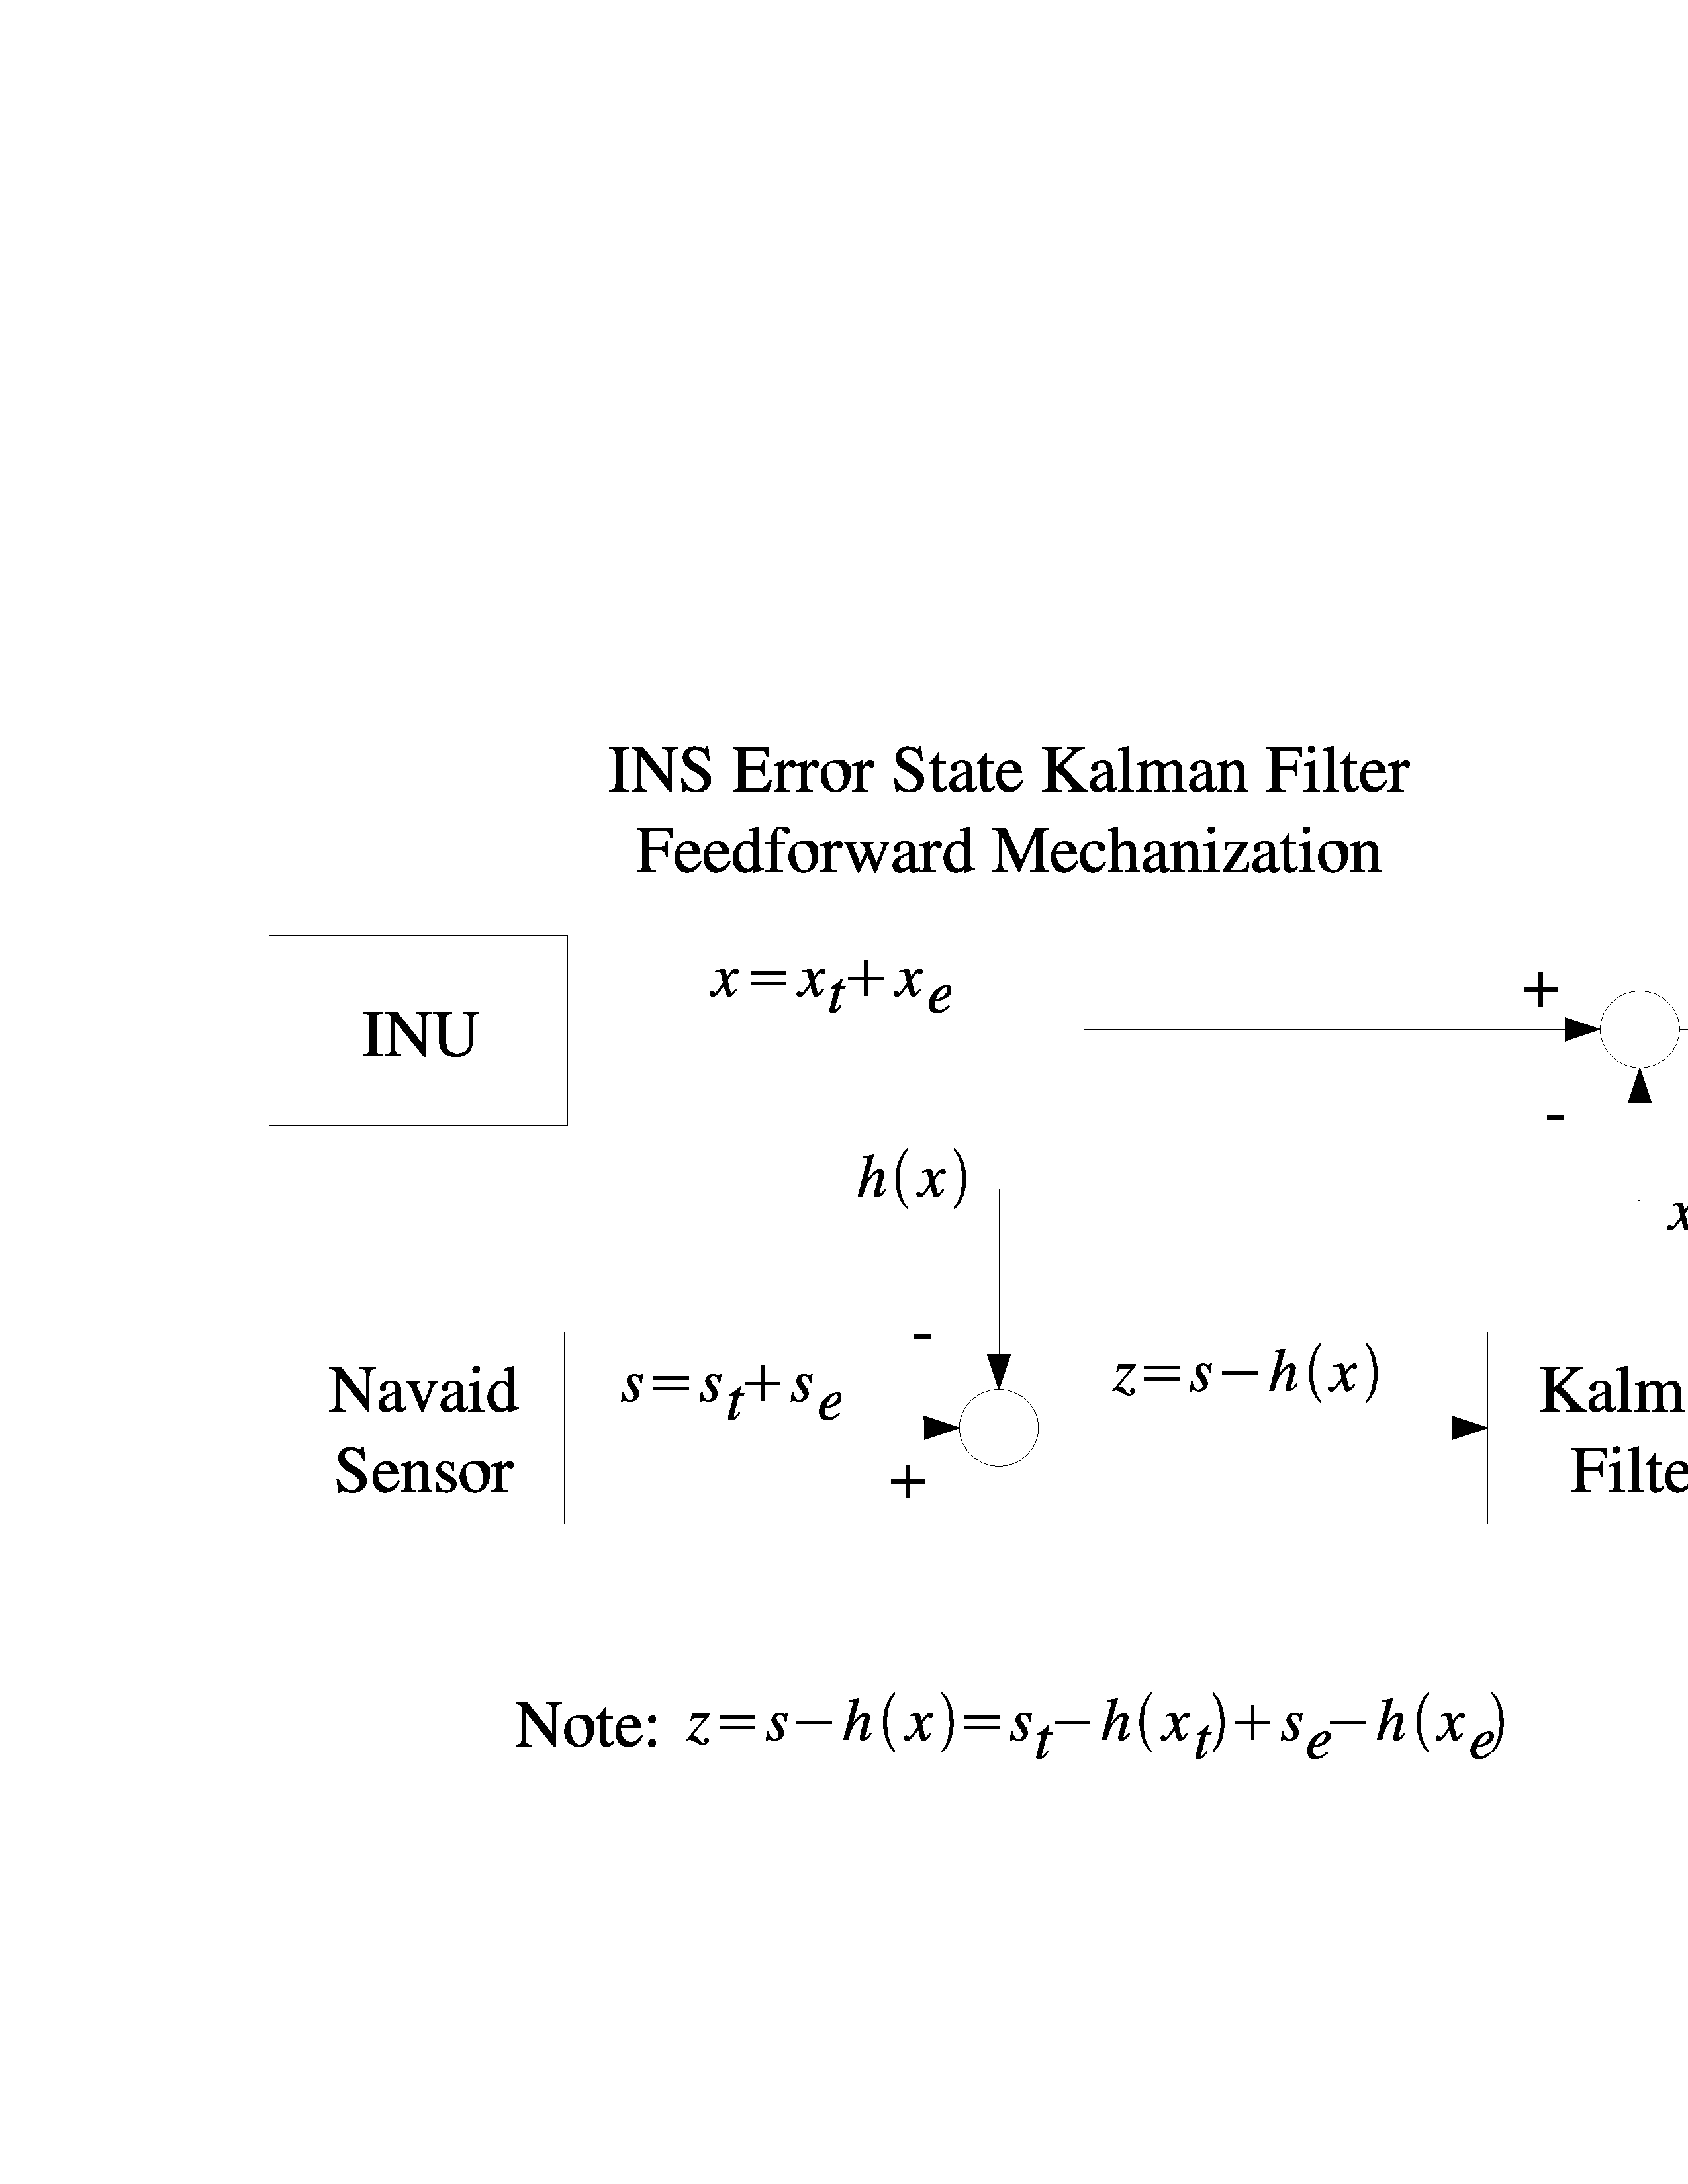
\includegraphics{day1_seg1_heuristic/feedforward.jpg}
\end{frame}

\begin{frame}
Navigation Aids (Navaids)
\begin{itemize}
  \item Measurement / Observation sources that aid in estimating INS error sources and dynamics
  \item Because we are interested in estimating INS errors, we use differencing to cancel out the whole state information
  \item INS outputs $x=x_t + x_e$, where $x_t$ is the true whole state information generated by INS, i.e., position, velocity, attitude, etc.
  \item Navaid sensor outputs $s=x_t+x_e$, where $x_t$ is once again the true quantities corrupted by sensor errors $x_e$.
\end{itemize} 
\end{frame}

\begin{frame}
Navigation Aids (Navaids)
\begin{itemize}
  \item Note that the navaid sensor usually only outputs part of the whole state vector, e.g., position and velocity, but not attitude (in the case of GPS)
  \item That's one reason why we have the $h$ function
  \item The INS signal is mapped by a linearized measurement function (or matrix) $h$ such that $h(x)=h(x_t) + h(x_e)$ and $h(x_t)=s_t$
\end{itemize} 
\end{frame}

\begin{frame}
Navigation Aids (Navaids)
\begin{itemize}
  \item Thus, we have
\begin{align*}
z&=s-h(x)\\
&=s_t + s_e - h(x_t) - h(x_e)\\
&=s_t - h(x_t) + s_e - h(x_e)\\
&=h(x_t) - h(x_t)+ s_e - h(x_e)\\
&=s_e - h(x_e)
\end{align*}
  \item Our measurement, therefore, is the difference between the navaid sensor errors and the INS errors
\end{itemize} 
\end{frame}

\begin{frame}
Navigation Aids (Navaids)
\begin{itemize}
  \item If $s_e$ is more than just white measurement noise, then we would need to model this vector in the filter according to known or assumed dynamics 
  \item Hence, sometimes adding a new navaid means adding new states to your filter

\end{itemize} 
\end{frame}

\begin{frame}
Navigation Aids (Navaids)
\begin{itemize}
  \item It is crucial to examine the innovations sequence for any non-white time correlations!
\[z_k-h\left[\stateest{k}{-}\right]=s_e(k)-h\left[(x_e(k)\right]-h\left[\stateest{k}{-}\right]\]
where we have added the index $k$ for clarity
 \item We should have $\expect{(z_k-h\left[\stateest{k}{-}\right])(z_j-h\left[\stateest{j}{-}\right])\trans}=0$ when $k\neq j$, which will in general be true provided $\expect{s_e(k)}=0$
 \item If this is not the case, then it is probably $s_e$ that is the culprit and you'd better start modeling!
\end{itemize} 
\end{frame}

\begin{frame}

\begin{itemize}
  \item The condition
\[\expect{(z_k-h\left[\stateest{k}{-}\right])(z_j-h\left[\stateest{j}{-}\right])\trans}=0
\]
says that the innovations sequence is uncorrelated in time.
  \item Recall that the innovations sequence is $\nu_k=z_k-h\left[\stateest{k}{-}\right]$
  \item Thus, we should have $\expect{\nu_k \nu_j\trans}=0$
  \item This means that the optimal estimator $\stateest{k}{+}$ always makes optimal use of the new information provided by $\nu_k$
\end{itemize} 
\end{frame}


% day4_seg2_navaids/gps.tex
\begin{frame}
GPS: The Global Positioning System
 \begin{itemize}
 \item 24+ satellites orbiting at 10,900 miles above surface
 \item Three Segments: Control, Space, User
 \item Time-tagged signals and known satellite position enable calculation of signal time of flight and hence range traversed from satellite to receiver
 \item Range to four satellites required to determine time plus three position coordinates
\end{itemize}
\end{frame}

\begin{frame}
GPS: The Global Positioning System
\begin{itemize}
  \item Satellites have precise atomic clocks
  \item User set receiver has less precise clock
  \item Time is of the essence:  comparing satellite-generated time-tag with user clock time of arrival determines transit time
  \item Note that user clock can be a source of systematic error
\end{itemize} 
\end{frame}

\begin{frame}
GPS: The Global Positioning System
\begin{itemize}
  \item Three types of navaid coupling:
  \begin{itemize}
	\item Loose coupling
    \item Tight coupling
    \item Deep coupling
  \end{itemize} 
\end{itemize} 
\end{frame}

\begin{frame}
Loosely-Coupled GPS
\begin{itemize}
  \item GPS receiver-generated position and velocity are differenced with INS position and velocity
  \item GPS position and velocity are generally pre-filtered (with a Kalman filter) before being used in inertial filter
  \item GPS position and velocity are also composite quantities from all satellites
  \item Least accurate approach to using GPS as a navaid
\end{itemize} 
\end{frame}

\begin{frame}
Loosely-Coupled GPS
\begin{itemize}
  \item The GPS receiver does not have the advantage of using inertial information to completely separate process noise from measurement noise
  \item Simplifies Kalman integration: Don't necessarily have to model GPS receiver clock errors (assume receiver has already done so)
\end{itemize} 
\end{frame}

\begin{frame}
Tightly-Coupled GPS
\begin{itemize}
  \item Pseudorange and delta pseudorange for each individual satellite are direct measurements presented to the filter
  \item Contains only measurement noise, not receiver filter's model of process noise 
  \item Gives INS filter more fine-grained control over GPS measurements
  \item Higher accuracy
\end{itemize} 
\end{frame}

\begin{frame}
Deeply-Coupled
\begin{itemize}
  \item Uses high-rate inertial data to aid in code and carrier phase tracking loops
  \item Most accurate solution when combined with tightly-coupled INS filter as well
\end{itemize} 
\end{frame}

\begin{frame}
GPS Errors
\begin{itemize}
  \item Ephemeris data: Satellite's reported position can be in error
  \item Satellite clock:  Negligible since SA (selective availability) has been turned off
  \item Ionosphere:  Pseudorange errors caused by free electrons in the ionosphere
\end{itemize} 
\end{frame}

\begin{frame}
GPS Errors (cont)
\begin{itemize}
  \item Troposphere: Pseudorange errors casued by temperature, pressure, humidity influences on the speed of light
  \item Multipath:  Errors casued by locking on to reflected signals
  \item Receiver Noise: Errors caused by receiver's thermal noise and software inaccuracies
\end{itemize} 
\end{frame}

\begin{frame}
\begin{center}
%\begin{tabular}{|c|p{2.5in}|p{2.5in} |} \hline
 \begin{tabular}{|p{3in}|p{1.5in}|p{1.5in}|} \hline
 % after \\ : \hline or \cline{col1-col2} \cline{col3-col4} ...
  \textbf{Error Source} & \textbf{C/A-Code Error Budget (meters)} & \textbf{P-Code Error Budget (meters)} \\ \hline
Multipath & 12.0 & 1.2 \\ \hline
Receiver Noise / Software & 11.1 & 1.1 \\ \hline
Ionosphereic Delays & 9.0 & 3.1 \\ \hline
Satellite Clock and  Ephemeris Errors & 3.9 & 3.9 \\ \hline
Tropspheric Delays & 2.0 & 2.0 \\ \hline
\end{tabular}
\end{center}
\end{frame}

\begin{frame}
Using Loosely-Coupled GPS Measurements
\begin{itemize}
  \item Position
	\begin{itemize}
		\item Form primary GPS position observation by subtracting Kalman-corrected INS reference position from raw GPS position
		\item Next, the innovation (or measurement residual) is formed by subtracting off the extrapolated state estimate of position error
		\item Extrapolated position error estimate needs to compensate for accumulated velocity error during Kalman cycle (or some fraction thereof) 
	\end{itemize}
\end{itemize} 
\end{frame}

\begin{frame}
An example (JOVIAL) from a transport aircraft navigation filter:
\end{frame}
\begin{verbatim}
  165  COMPUTE RESIDUALS 
  166      RESIDUALS(1) = Y'KAL'OBS(INU,1) * OBS'COUNT'SCALER - SVVAR(1)
  167 	- 5.0 * SVVAR(4);
  168      RESIDUALS(2) = Y'KAL'OBS(INU,2) * OBS'COUNT'SCALER - SVVAR(2)
  169 	- 5.0 * SVVAR(5);
  170      RESIDUALS(3) = Y'KAL'OBS(INU,7) * OBS'COUNT'SCALER - SVVAR(3)     
  171         - 5.0 * SVVAR(6);

\end{verbatim}

\begin{frame}
GPS Velocity Measurements
\begin{itemize}
  \item Based on carrier phase measurements in receiver
  \item Generally independent of position measurements
  \item Observation is once again difference between Kalman-compensated INS reference velocity and GPS-indicated velocity
\end{itemize} 
\end{frame}

\begin{frame}
GPS Measurment Noise Covariance
\begin{itemize}
  \item Based on EHE (estimated horizontal error) and EVE (estimated vertical error)
  \item These numbers highgly dependent on GDOPs
\end{itemize} 
\end{frame}

\begin{frame}
Geometric Dillution of Precision (GDOP)
\begin{itemize}
  \item Satellites are not geostationary
  \item H matrix is time-varying
  \item Observability varies with time
  \item $GDOP=\sqrt{\text{tr}\left(H\trans H\right)^{-1}}$
\end{itemize} 
\end{frame}


\begin{frame}
GDOP Chimney
\begin{itemize}
  \item Large DGOP is bad; normal values 3-5
  \item Singularity periods of time (about 1 hr) when GDOP values spike upward with a peak as much as 1000
  \item GDOP 50 $\approx$ 500 m position error
  \item Chimney's effects should be less acute if receiver has enough channels to track many satellites and to handle constellation changes
\end{itemize} 
\end{frame}


% day4_seg2_navaids/posfix.tex
\begin{frame}
Position Fix
 \begin{itemize}
 \item Overfly Fix
 \item Known location
 \item Delta formed between overfly location and indicated, Kalman-compensated INS position
 \item Usually a one-shot opportunity, i.e., not periodic like GPS
\end{itemize}
\end{frame}

% day4_seg2_navaids/radar.tex
\begin{frame}
Radar Fixes
 \begin{itemize}
 \item Instantaneous azimuth and elevation angles to a target of known latitude and longitude
 \item Or converted to local Cartesian coordinates (north, east, and altitude)
 \item Amount of cursor movement required to align curson with target yields position fix delta
 \item Otherwise, processed in filter like GPS or visual position fix
\end{itemize}
\end{frame}

% day4_seg2_navaids/dvs.tex
\begin{frame}
Doppler Velocity Sensor (DVS)
 \begin{itemize}
 \item DVS provides genuine velocity measurement with respect to ground
 \item DVS provides heading and drift velocities $V_H$ and $V_D$
 \item Nonlinear measurement relationship to INS-indicated velocities $V_x$ and $V_y$ and platform azimuth $\beta$:
\end{itemize}
\begin{align*}
V_H &= -V_x\sin\beta + V_y\cos\beta\\
V_D &=  V_x\cos\beta + V_y\sin\beta
\end{align*}
\end{frame}

\begin{frame}
DVS
\begin{itemize}
  \item Relationship between $(V_x,V_y)$ and $(V_H,V_D)$ is non-linear $h$
  \item To generate a linearized $H$ matrix we compute partial derivatives (Jacobians) to yield:
\[H=
\begin{bmatrix}
0&-\sin\beta&0&0&\cos\beta&0&0&0&-V_x\cos\beta - V_y\sin\beta\\
0&\cos\beta&0&0&\sin\beta&0&0&0&-V_x\sin\beta + V_y\cos\beta
\end{bmatrix}
\]
for a canonical 9-state filter.
\end{itemize} 
\end{frame}

% day4_seg2_navaids/tracking.tex
\begin{frame}
External Tracking Aids
 \begin{itemize}
 \item External platform tracks your vehicle and sends position / velocity info (JTIDS) 
 \item Bearing and distance measurments
	\begin{itemize}
		\item VOR, DME, TACAN
	\end{itemize}
\end{itemize}
\end{frame}

%% day4_seg2_navaids/att.tex
\begin{frame}
Attitude References
 \begin{itemize}
 \item 
 \item
 \item
\end{itemize}
\end{frame}

% day4_seg2_navaids/dted.tex
\begin{frame}
Digital Terrain Elevation Data (DTED)
 \begin{itemize}
 \item Published by National Geospatial Intelligence Agency (NGA)
	\begin{itemize}
		\item formerly NIMA, formerly DMA
	\end{itemize}
 \item 1 deg geocells of terrain height for each lat/long pair
 \item DTED Levels 0,1,2
\end{itemize}
\end{frame}

\begin{frame}
DTED
\begin{itemize}
  \item As navaid, a trail of radar altimeter measurements are stored
  \item Trail is correlated with DTED to determine offset
  \item SITAN, TERPROM
\end{itemize} 
\end{frame}

%% day4_seg2_navaids/exercises.tex
\begin{frame}
Exercises
 \begin{itemize}
 \item
 \item
 \item
\end{itemize}
\end{frame}


% day4_seg3_maint/maint_main.tex
\begin{frame}
\textbf{Day 4, Segment 3\\
Filter Maintenance\\
Topics}
 \begin{itemize}
 \item Filter Performance and Integrity Monitoring
 \item Replacing Navaids
 \item Adding New Navaids
 \item Augmenting the State Vector
\end{itemize}
\end{frame}
% day4_seg3_maint/perf_integ.tex
\begin{frame}
Filter Performance and Integrity Monitoring
 \begin{itemize}
 \item Covariance Monitoring
 \item Innovations Monitoring
 \item Corrective Action
\end{itemize}
\end{frame}
\begin{frame}
Covariance Monitoring
\begin{itemize}
  \item Ensuring Symmetry
  \item Managing Observability
  \item Ensuring Positive Definiteness
\end{itemize} 
\end{frame}
\begin{frame}
Covariance Monitoring:  Ensuring Symmetry
\begin{itemize}
  \item $P$ is supposed to be positive definite and symmetric
  \item Symmetry means that $P\trans = P$, i.e., for each element $p_{ij}$ of $P$ we must have $p_{ij}=p_{ji}$
  \item Roundoff error can cause loss of symmetry
  \item The best way to ensure symmetry is to work only with items on or (say) above the diagonal and simply define elements below he diagonal by fiat.
\end{itemize} 
\end{frame}
\begin{frame}
Covariance Monitoring:  Ensuring Symmetry
\begin{itemize}
  \item Both $P(+)$ and $P(-)$ need to be symmetrized
\begin{itemize}
  \item After extrapolation: symmetrize
  \item After update: symmetrize
\end{itemize}
\end{itemize} 
\end{frame}
\begin{frame}
Covariance Monitoring:  Managing Observability
\begin{itemize}
  \item Observability means there is a linear path from the measurements to states
  \item Structural observability determined by $\Phi$ and $H$:
\end{itemize}
 If $H$ is $1\times n$, where $n$ is the size of the state vector, then the state $x_0$ is said to be \textbf{observable }from $n$ scalar measurements $\set{z_0,\ldots,z_{n-1}}$ if the block matrix
\[
\begin{bmatrix}
H\trans&\Phi\trans H\trans & \cdots & (\Phi\trans)^{n-1}H\trans
\end{bmatrix}
\]
is of rank $n$
\end{frame}
\begin{frame}
Covariance Monitoring:  Managing Observability
\begin{itemize}
  \item If unobservable states are also unstable, estimation errors will be unstable and $P$ will show symptoms 
\begin{itemize}
  \item $\text{diag}(P)\rightarrow \infty$
  \item I.e., one or more diagonal elements of $P$ will grow without bound
\end{itemize}
  \item Not the same as divergence: "feature" of the design
\end{itemize}
\end{frame}
\begin{frame}
Covariance Monitoring:  Managing Observability
\begin{itemize}
  \item Note also that the state estimation error variances (i.e., the diagonals of $P$) will naturally grow in the absence of measurements
  \item Going for a long time without incorporating a measurement is equivalent to lack of observability in the associated states
  \item Use covariance analysis simulation to detect non-observability
  \item The only real solution is to add new measurements
\end{itemize}
\end{frame}
\begin{frame}
Covariance Monitoring:  Ensuring Positive Definiteness
\begin{itemize}
  \item $P$ is supposed to be positive definite
  \item This means that $x'Px>0$ whenever $x\neq0$
  \item States modeled as random constants or other deterministic states can cause loss of positivity
  \item Add covariance bumping:  Add small amounts of process noise to diagonal elements of $Q$ for these states
\end{itemize}
\end{frame}

% day4_seg3_maint/replace_navaids.tex
\begin{frame}
Replacing Navaids
 \begin{itemize}
 \item Replacing a given sensor with another of the same type usually requires no changes to the state model
	\begin{itemize}
		\item unless replacement sensor has significant errory dynamics that need to be modeled (see adding new sensors and state augmentation)
	\end{itemize}
 \item Measurement noise covariance generally has to change however
\end{itemize}
\end{frame}

% day4_seg3_maint/new_navaids.tex
\begin{frame}
Adding New Navaids
 \begin{itemize}
 \item What kinds of navaids are desirable?
 \item What are the steps involved in adding a new navaid?
\end{itemize}
\end{frame}
\begin{frame}
Adding New Navaids\\
Desirable Characteristics:
\begin{itemize}
  \item Navaids which render observable otherwise unobservable states
  \item Those having a simple relationship (preferably linear) to the state vector
  \item Having only white noise error dynamics
\end{itemize} 
\end{frame}

% day4_seg3_maint/aug_state_vec.tex
\begin{frame}
Augmenting the State Vector
 \begin{itemize}
 \item State Vector Augmentation: Expanding the size of the state vector
\begin{itemize}
	\item i.e., adding new states
\end{itemize}
 \item Why?
\begin{itemize}
	\item new navaids with their own error dynamics (e.g., GPS)
	\item correlated (non-white) process noise
	\item correlated (non-white) measurement noise
\end{itemize}
\end{itemize}
\end{frame}
\begin{frame}
Augmenting the State Vector
\begin{itemize}
  \item Why? (continued)
\begin{itemize}
  \item Correlation $\Rightarrow$ dynamics
\begin{itemize}
	\item No dynamics in white noise
\end{itemize}
  \item If dynamics are present they must be modeled
  \item Otherwise, dynamic effects will be allocated to other states
\end{itemize} 
\end{itemize} 
\end{frame}
\begin{frame}
Augmenting the State Vector
\begin{itemize}
 \item How?
\begin{itemize}
	\item model non-white noise as result of feeding white noise through a linear system
	\item new states are outputs of new integrators
\end{itemize}
  \item State transition matrix $\Phi$ and error covariance matrix $P$ grow as $j^2$, where $j$ is number of new states
  \item Geometry matrix $H$ grows as $m\cdot j$, where $m$ is number of measurements and $j$ is number of new states
\end{itemize} 
\end{frame}
\begin{frame}
Augmenting the State Vector\\
Example: Ship Inertial Navigation Systems (SINS)
\begin{itemize}
  \item Long mission times
\begin{itemize}
	\item Especially submarines
\end{itemize}
  \item Position fixes insufficient to calibrate gyro bias drift w/o further modeling
\end{itemize} 
\end{frame}
\begin{frame}
Augmenting the State Vector\\
Example: Ship Inertial Navigation Systems (SINS)
\begin{itemize}
  \item Gyro bias drift due to slowly changing bias
  \item Can be modeled as random walk
  \item Random walk modeled as integrated white noise
  \item Kalman filter needed to estimate drift 
\end{itemize} 
\end{frame}
\begin{frame}
Augmenting the State Vector\\
Example: Ship Inertial Navigation Systems (SINS)
\begin{itemize}
  \item Assume platform tilts are kept close to zero through velocity measurements damping the Schuler oscillations
  \item North-West-Up (NWU) coordinate frame (or West-South-Up)
\end{itemize} 
\end{frame}
\begin{frame}
Augmenting the State Vector\\
Example: Ship Inertial Navigation Systems (SINS)
\begin{itemize}
  \item Two angular position errors in radians:  $\psi_N$ and $\psi_W$
\begin{itemize}
	\item Note $\psi_N$ is a small angular rotation about the north axis and  thus induces a west position error.
    \item Similarly, $\psi_W$ is a small rotation about the west axis and thus induces a south position error.
\end{itemize}
  \item $\theta_U =\psi_Z - \psi_N \tan(\lambda)$, where $\psi_Z$ is platform azimuth error and $\lambda$ is the latitude.
\end{itemize} 
\end{frame}
\begin{frame}
Augmenting the State Vector\\
Example: Ship Inertial Navigation Systems (SINS)
\begin{itemize}
  \item Error Dynamics:
\begin{align*}
\dot{\psi}_N - \Omega_U\psi_W &= \delta g_N\\
\dot{\psi}_W + \Omega_U \psi_N - \Omega_N\theta_U &= \delta g_W\\
\dot{\theta}_U + \Omega_N \psi_W &= \delta g_U
\end{align*}
where $\delta g_N,\delta g_W,\delta g_U$ are non-white gyro bias drift errors and $\Omega_N=\Omega\cos(\lambda)$ and $\Omega_U=\Omega\sin(\lambda)$ are components of earth rate
\end{itemize} 
\end{frame}
\begin{frame}
Augmenting the State Vector\\
Example: Ship Inertial Navigation Systems (SINS)
\begin{itemize}
  \item Since $\delta g_N,\delta g_W,\delta g_U$ are non-white, the question arises as to what kind of model is appropriate
  \item Empirical data indicates that gyro biases exhibit random walk behavior over time
  \item Since random walk is the integral of white noise, white noise can be viewed (in some sense) as the derivative of random walk
\end{itemize} 
\end{frame}
\begin{frame}
Augmenting the State Vector\\
Example: Ship Inertial Navigation Systems (SINS)
\begin{itemize}
  \item Hence, the following dynamics of random walk apply:
\begin{align*}
\dot{\delta} g_N &= w_N\\
\dot{\delta} g_W &= w_W\\
\dot{\delta} g_U &= w_U
\end{align*}
where $w_N,w_W,w_U$ are white noise processes.
\end{itemize} 
\end{frame}
\begin{frame}
Augmenting the State Vector\\
Example: Ship Inertial Navigation Systems (SINS)
\begin{itemize}
  \item We use the random walk equations to augment the state dynamics equations
  \item Thus we now have a six-state model:
\end{itemize} 
\[
\begin{bmatrix}
\dot{\psi}_N\\
\dot{\psi}_W\\
\dot{\theta}_U\\
\dot{\delta} g_N\\
\dot{\delta} g_W\\
\dot{\delta} g_U
\end{bmatrix}
=
\begin{bmatrix}
0&\Omega_U&0&1&0&0\\
-\Omega_U&0&\Omega_N&0&1&0\\
0&-\Omega_N&0&0&0&1\\
0&0&0&0&0&0\\
0&0&0&0&0&0\\
0&0&0&0&0&0
\end{bmatrix}
\begin{bmatrix}
\psi_N\\
\psi_W\\
\theta_U\\
\delta g_N\\
\delta g_W\\
\delta g_U
\end{bmatrix}
+\begin{bmatrix}
0&0&0&0&0&0\\
0&0&0&0&0&0\\
0&0&0&0&0&0\\
0&0&0&1&0&0\\
0&0&0&0&1&0\\
0&0&0&0&0&1
\end{bmatrix}
\begin{bmatrix}
0\\
0\\
0\\
w_N\\
w_W\\
w_U
\end{bmatrix}
\]
\end{frame}
\begin{frame}
Augmenting the State Vector:  Summary
\begin{itemize}
  \item Straightforward: When new, relevant dynamic relations found, simply add the states to the state vector and add the new dynamics to the $F$ and/or $\Phi$ matrix
  \item Use basic models such as low-order systems driven by white noise to model new states
\end{itemize}
\end{frame}
\begin{frame}
Augmenting the State Vector:  Summary
\begin{itemize}
  \item Some Popular Models
\begin{itemize}
	\item random walk
	\item random constant
	\item random ramp
	\item Gauss-Markov (i.e., exponentially correlated)
	\item combinations of the above!
\end{itemize}
\end{itemize} 
\end{frame}


% day4_seg3_maint/exercises.tex
\begin{frame}
Exercises
 \begin{enumerate}
 \item Write a simple 1-state model for a gyro bias modeled as a random constant
 \item Now augment this model to a 2-state model by adding a random walk
\end{enumerate}
\end{frame}


% day4_seg4_redund/redund_main.tex
\begin{frame}
\textbf{Day 4, Segment 4\\
Filter Redundancy and Fault Tolerance\\
Topics}
 \begin{itemize}
 \item Typical Weighting Scheme
 \item Detecting Faults
 \item Graceful Degradation
\end{itemize}
\end{frame}
% day4_seg4_redund/ct_weighting.tex
\begin{frame}
Typical Weighting Scheme
 \begin{itemize}
 \item Two separate INS error dynamics filters
 \item Use error covariance outputs from each filter to weight state estimates
\end{itemize}
\end{frame}

\begin{frame}
Typical Weighting Scheme
 \begin{itemize}
 \item Weighting scheme:
\[w_i(x)=\dfrac{\sigma_j(x)}{\sigma_1(x)+\sigma_2(x)}\]
where $i\neq j\in\set{1,2}$ and $x$ is the parameter in question
\end{itemize}
\end{frame}

\begin{frame}
Alternatives to Weighting: Decentralized Filtering
\begin{itemize}
  \item Decentralized filtering without feedback
  \item Decentralized filtering with feedback
\end{itemize} 
\end{frame}

\begin{frame}
Decentralized Filtering without Feedback
\begin{itemize}
  \item Assume two local filters
  \item Then for the global error covariance we have:
\[P^{-1}=P_1^{-1}+M_1^{-1}+P_2^{-1}+M_2^{-1}+M^{-1}\]
where $P_1,P_2$ are updated local error covariances for each filter, $M_1,M_2$ are extrapolated local error covariances prior to update, and $M$ is the global filter's prior error covariance.
\end{itemize} 
\end{frame}

\begin{frame}
Decentralized Filtering without Feedback
\begin{itemize}
  \item The global filter's estimate is
\[\hat{x}=P\left[P_1^{-1}\hat{x}_1-M_1m_1^{-1}+P_2^{-1}\hat{x}_2-M_2m_2^{-1}+M^{-1}m\right]\]
where $m_1,m_2,m$ are the local a priori estimates for local filters 1 and 2 and the global filter, respectively.
\end{itemize} 
\end{frame}

%% day4_seg4_redund/fault_detection.tex
\begin{frame}
Detecting Faults
 \begin{itemize}
 \item
 \item
 \item
\end{itemize}
\end{frame}

%% day4_seg4_redund/graceful_deg.tex
\begin{frame}
Graceful Degradation
 \begin{itemize}
 \item
 \item
 \item
\end{itemize}
\end{frame}

% day4_seg4_redund/exercises.tex
\begin{frame}
Exercises
 \begin{enumerate}
 \item Let the x position error variance for filter 1 be 4 meters, that of filter 2 16 meters.  Calculate the weighted average latitude given lat1=33.3 deg, lat2=33.21.   
 \item How would the decentralized filter's estimate differ from the weighted average?
\end{enumerate}
\end{frame}


% ----------------------------------------------------------------
\end{document}
